\documentclass[11pt,usenames,dvipsnames,svgnames,x11names]{beamer} 

\usetheme{Warsaw}
\usepackage{amssymb,amsmath,amsthm,amsfonts}                    
\usecolortheme{whale} 
\setbeamertemplate{navigation symbols}{}
\usepackage[utf8]{inputenc} 
\usepackage{polski}
\usepackage{tikz}
\usepackage{subfigure}
\usepackage{setspace}
\usepackage{savesym}
\savesymbol{arc}
\usepackage{color}
\usepackage{xcolor}
\usepackage{pict2e}
\usepackage{epstopdf}
\usepackage{caption}

\date{14 stycznia 2014}
\author{Zofia Plackowska i Marta Sommer}
\title{Karty kontrolne wartości średniej i odchylenia standardowego}

\theoremstyle{plain}
\newtheorem{twierdzenie}{Twierdzenie} 
\newtheorem{twierdzeniecd}{Twierdzenie cd.} 
\theoremstyle{definition}
\newtheorem{definicja}{Definicja}
\newtheorem{przyklad}{Przykład}
\newtheorem{lemat}{Lemat}
\newtheorem{wniosek}{Wniosek}
\newtheorem{oznaczenia}{Oznaczenia}
\theoremstyle{remark}
\newtheorem{uwaga}{Uwaga}

%\setbeamercovered{transparent}

\begin{document}


\begin{frame}   %tytułowa
\titlepage
\end{frame}

%%%%%%%%%%%%%%%%%%%%%%%%%%%%%%%%%%%%%%%%%%%%%%%%%%%%%%%%%%%%%%%%%%%%%%%%%%%%%%%%%%%%%%%%%%%%%%%%%%%%%%%%%%%%%%%%%%%%%

\begin{frame}
\frametitle{SSP - wprowadzenie}
SSP składa się z trzech zasadniczych kroków:
\begin{enumerate}
\item sporządzenie dokładnego diagramu procesu produkcji,
\item pobieranie losowych próbek i dokonywanie na nich pomiarów w regularnych odstępach czasu i na wielu etapach procesu produkcji,
\item użycie zaobserwowanych przypadków rozregulowania procesu (na danym etapie) do wykrycia ich przyczyn, tak by można było te przyczyny usunąć. 
\end{enumerate} 
\end{frame}

\begin{frame}
\frametitle{SSP - wprowadzenie}
Główne założenia:
\begin{enumerate}
\item maszyny nie zachowują się jak ludzie
\item celem nie jest pracowanie ciężko, lecz inteligentnie
\item SSP to nie to samo, co kontrola odbiorcza
\item etapowa, stała poprawa jakości 
\end{enumerate}
\end{frame}


%%%%%%%%%%%%%%%%%%%%%%%%%%%%%%%%%%%%%%%%%%%%%%%%%%%%%%%%%%%%%%%%%%%%%%%%%%%%%%%%%%%%%%%%%%%%%%%%%%%%%%%%%%%%%%%%%%%%%

\begin{frame}   
\frametitle{Proces z dryfem wartości oczekiwanej}
	
Rozważmy przykład związany z~produkcją śrub. Załóżmy,~że w~chwili $t$, pobrana próbka ma rozkład $\mathcal{N}(\mu_t,\sigma^2)$ oraz że wartość~$\mu_t$ zmienia się w~czasie ("dryfuje"), zgodnie z~poniższym równaniem rekurencyjnym $$\mu_t=\mu_{t-1}+\epsilon_t,$$gdzie $\epsilon_t$ jest zmienną losową o~wartości oczekiwanej $0$ i~wariancji~$\tau^2$. 
	
\end{frame}

\begin{frame} 
\frametitle{Proces z dryfem wartości oczekiwanej}

Dla symulacji z parametrami: $\mu_1=10$, $\sigma=0.1$ oraz $\tau=0.01$, otrzymujemy następujące karty kontrolne wartości średniej:

\begin{center}
	\begin{figure}[htbp]
			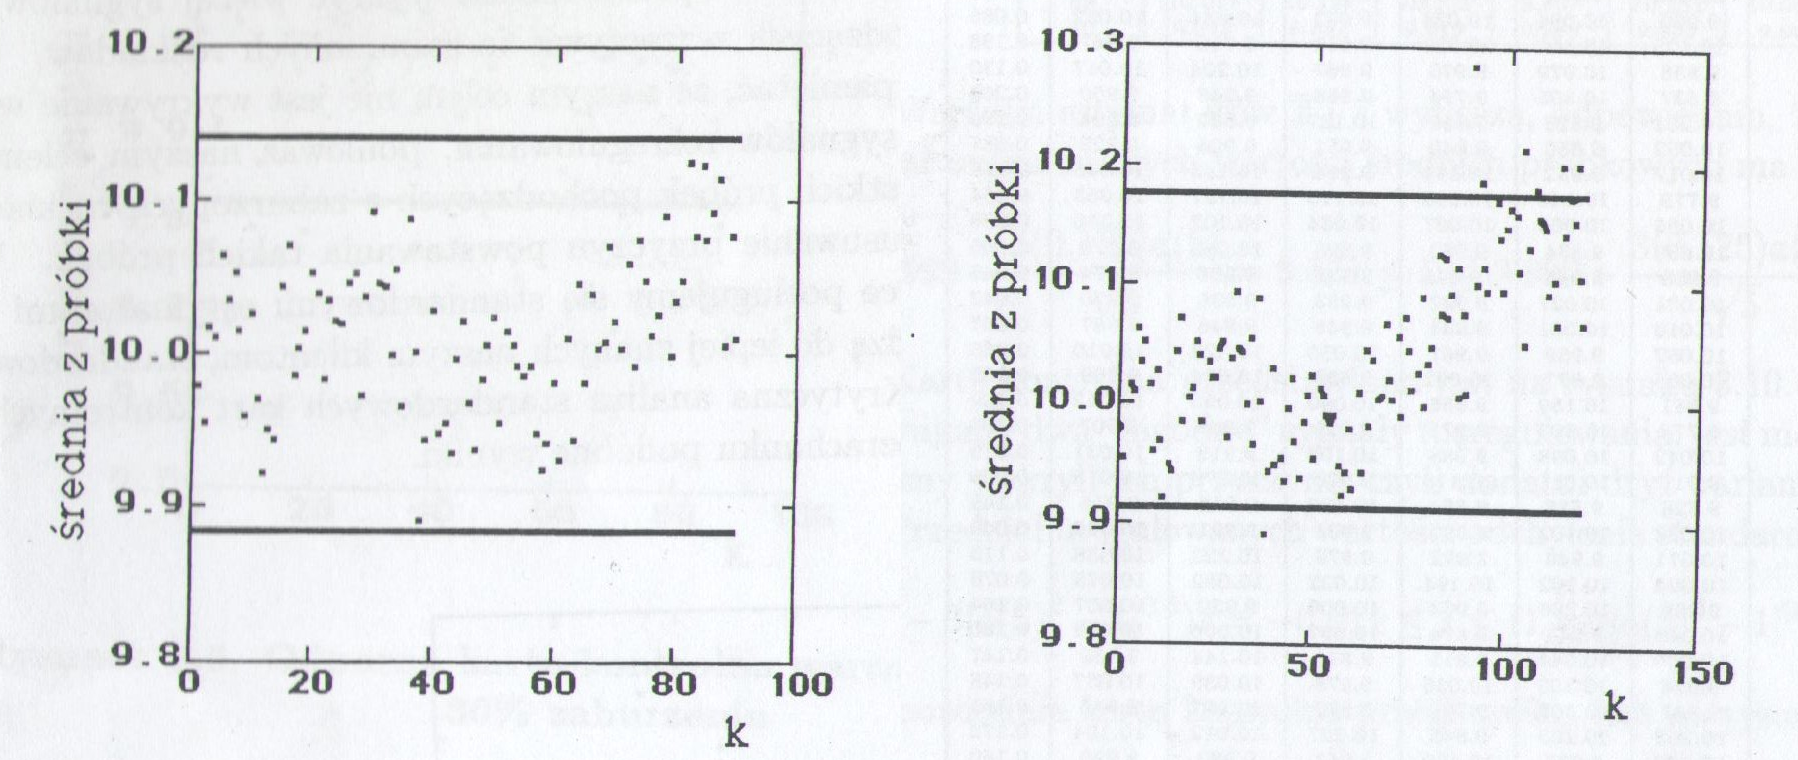
\includegraphics[width=\textwidth]{obr1.png}
			\caption{Karta kontrolna wartości średniej przy dryfie średniej}
	\end{figure}
\end{center}

\end{frame}

\begin{frame} 
\frametitle{Karta kontrolna różnic wartości średnich}

Zbudujmy następujący model:
$$x_{t,j}=\mu_t+\eta_{t,j},$$
gdzie $j=1,\dots,n$, $\eta_{t,j}\sim\mathcal{N}(0,\sigma^2)$ oraz 
$$\mu_t=\mu_{t-1}+\epsilon_t,$$gdzie $\epsilon_t\sim\mathcal{N}(0,\tau^2)$.
Wówczas definiujemy różnicę między $(t+1)$-szą i $t$-tą średnią:
$$\Delta=\overline{x}_{t+1}-\overline{x}_{t}.$$
Możemy dla niej skonstruować kartę kontrolną wartości średnich. 
\end{frame}

\begin{frame}
\frametitle{Karta kontrolna różnic wartości średnich}
\begin{center}
	\begin{figure}[htbp]
			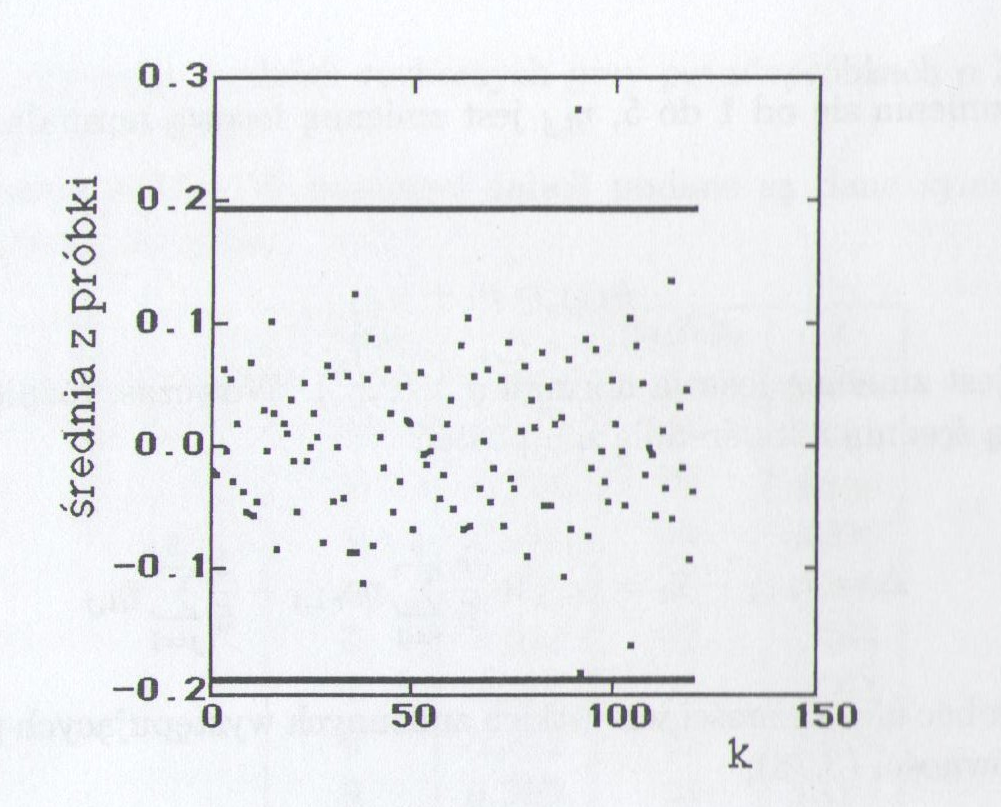
\includegraphics[width=0.8\textwidth]{obr2.png}
			\caption{Karta kontrolna różnic wartości średnich przy dryfie średniej}
	\end{figure}
\end{center}
\end{frame}

\begin{frame} 
\frametitle{Proces z dodatnim dryfem wariancji}

\begin{center}
	\begin{figure}[htbp]
			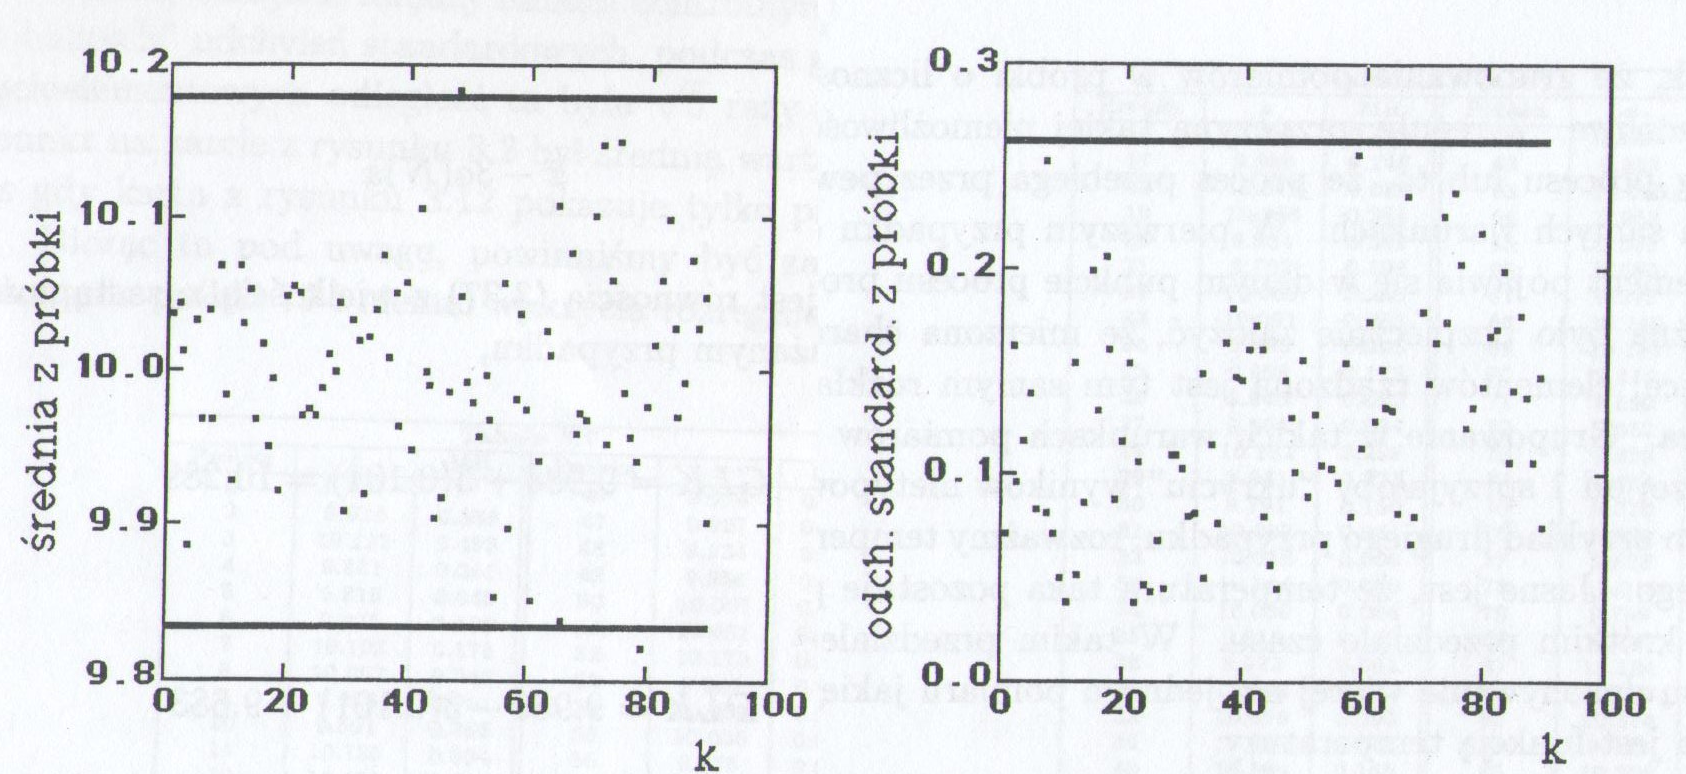
\includegraphics[width=\textwidth]{obr3.png}
			\caption{Karta kontrolna wartości średniej i odchylenia standardowego przy dryfie wariancji}
	\end{figure}
\end{center}
\end{frame}

\begin{frame}
\frametitle{Karty kontrolne dla pojedynczych pomiarów}

Zamiast średnich próbkowych umieszczamy wyniki pomiarów, a~zamiast średniej odchyleń standardowych wyznaczamy odchylenie standardowe wszystkich pomiarów. GLK i~DLK wyznaczamy więc z~następującego wzoru:
$$\overline{x}\pm3a(N)s,$$
gdzie $a(N)$ wyznaczamy jak~w przypadku zwykłej karty kontrolnej~z wielkością $n$ zastąpioną przez $N$.

\end{frame}

\begin{frame}
\frametitle{Karty kontrolne dla pojedynczych pomiarów}
\begin{center}
	\begin{figure}[htbp]
			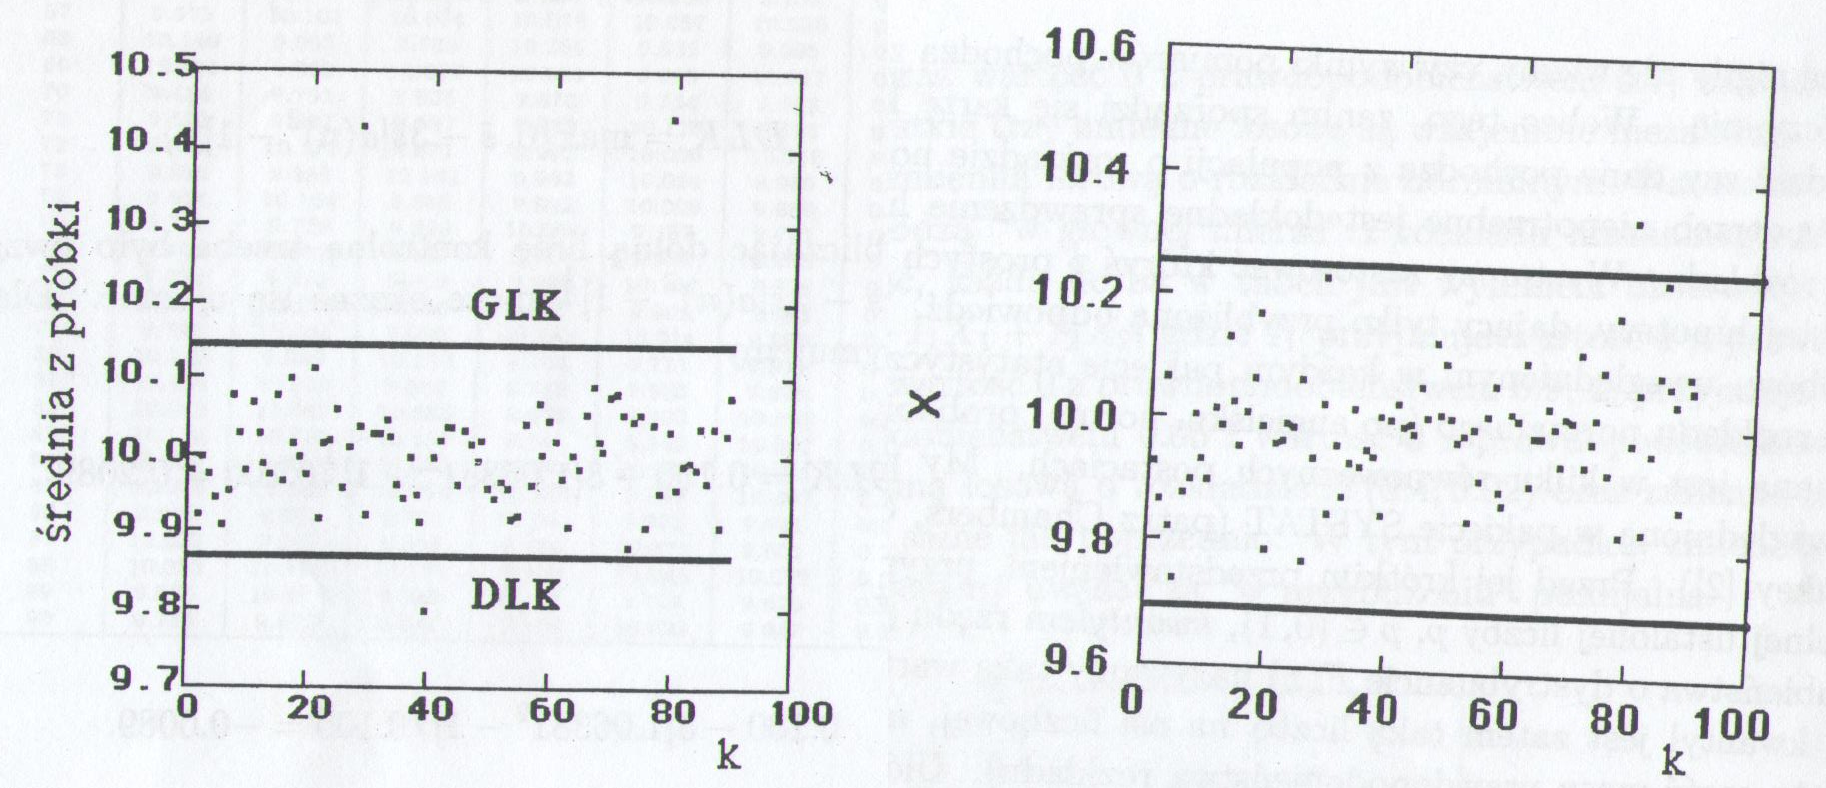
\includegraphics[width=\textwidth]{obr4.png}
			\caption{Zwykła karta kontrolna wartości średnich oraz karta kontrolna wartości średnich pojedynczych pomiarów}
	\end{figure}
\end{center}
\end{frame}

\begin{frame}
\frametitle{Sprawdzanie normalności rozkładów}

Stosujemy tu tzw. siatkę rozkładu normalnego.

\begin{center}
	\begin{figure}[htbp]
			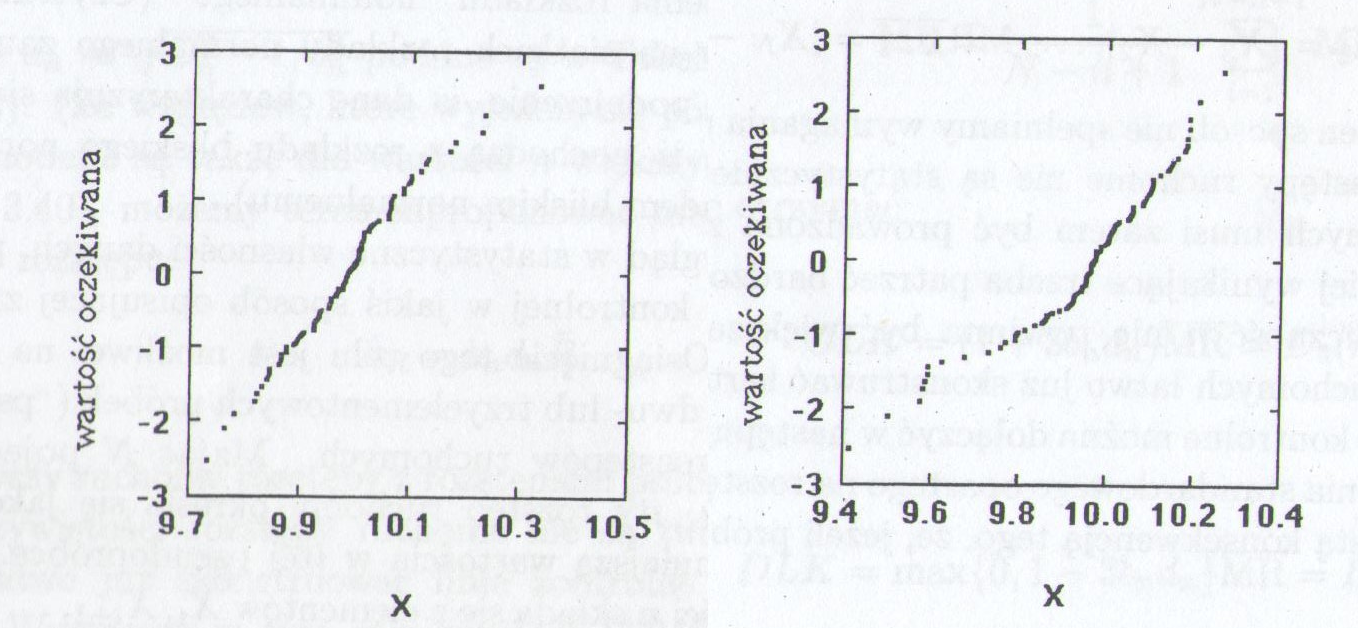
\includegraphics[width=\textwidth]{obr5.png}
			\caption{Dwie siatki rozkładu normalnego - pierwszy rozkład jest normalny, a drugi nie}
	\end{figure}
\end{center}
\end{frame}

\begin{frame}
\frametitle{Rozstępy ruchome}

Mamy $N$ pojedynczych obserwacji: $X_1,\ldots,X_N$. $i$-ty \textbf{rozstęp ruchomy} określa się jako różnicę między największą i~najmniejszą wartością w~tzw.~$i$-tej~pseudopróbce. Z~kolei $i$-ta pseudopróbka o~liczności $n$ składa się z~elementów $X_i,X_{i+1},\ldots,X_{i+n-1}$, gdzie $i=1,2,\ldots,N-n+1$. Zwykle przyjmuje się liczność pseudopróbki $2$ lub $3$. Więc, jeśli $n=2$ mamy:
$$MR_1=|X_2-X_1|, MR_2=|X_3-X_2|,\ldots,MR_{N-1}=|X_N-X_{N-1}|$$
Linie kontrolne dla karty rozstępu ruchomego konstruuje się przyjmując za~GLK i~DLK następujące wartości:
$$GLK=D_4(n)\overline{MR}$$
$$DLK=D_3(n)\overline{MR},$$
gdzie $D_3(n)$ i $D_4(n)$ są to pewne stałe.

\end{frame}

\begin{frame}
\frametitle{Wydolność procesu}

Miary wydolności procesu:
\begin{itemize}
\item wskaźnik zdolności: $$C_p=\frac{T_g-T_d}{6\hat{\sigma}},$$ gdzie $T_g, T_d$ - odpowiednio górna i~dolna granica tolerancji
\item wskaźnik wydajności: $$C_{pk}=\frac{Z_{min}}{3},$$ gdzie $Z_{min}=\min\lbrace Z_{T_g},-Z_{T_d}\rbrace$ oraz $Z_{T_g}=\frac{T_g-\overline{\overline{x}}}{\hat{\sigma}}$ i $Z_{T_d}=\frac{T_d-\overline{\overline{x}}}{\hat{\sigma}}$
\end{itemize}


\end{frame}

\begin{frame}
\frametitle{Bibliografia}
\begin{thebibliography}{9}
\bibitem{HM} J. Koronacki: \emph{Statystyczne sterowanie procesem. Metoda Deminga etapowej optymalizacji jakości},  Akademicka Oficyna Wydawnicza PLJ, Warszawa 1994
\end{thebibliography}
\end{frame}


\begin{frame}  
\frametitle{~}
\begin{center}
\Large{Dziękujemy za uwagę}
\end{center}

\end{frame}


\end{document}
